\section{approach}
\label{sec:approach}
In this section, we first formulate the just-in-time defect prediction and provide an overview of our framework. We then describe the details of each part inside the framework. Finally, we present an algorithm for learning effective settings of our model's parameters. 
\subsection{Framework Overview}
\label{sec:overview}

\begin{figure}
\center
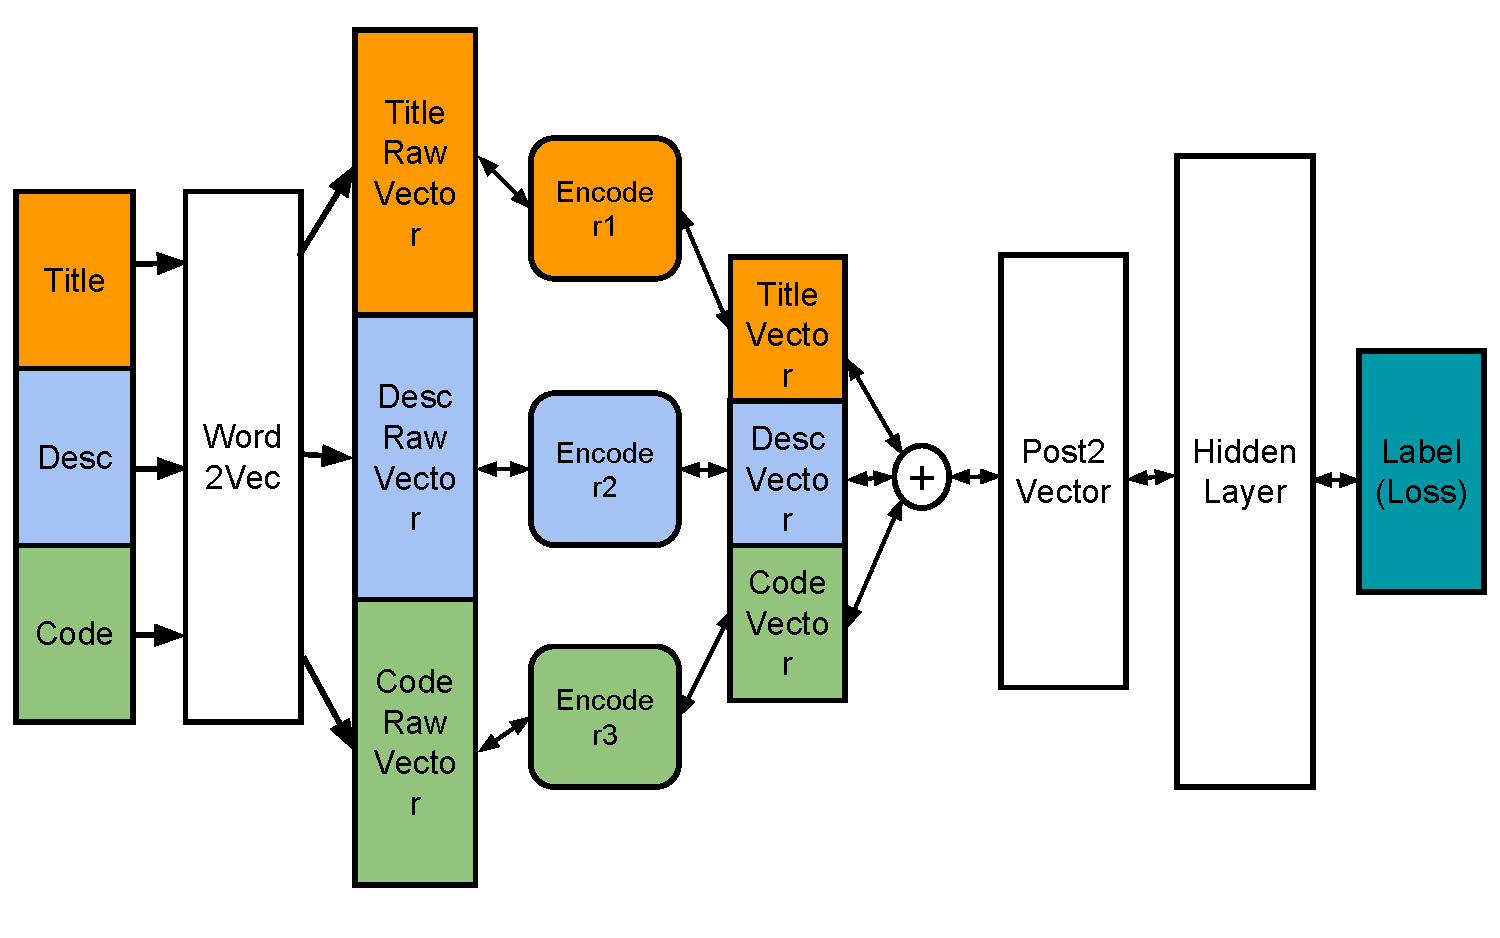
\includegraphics[scale=0.36]{figs/framework.pdf}
\caption{The general framework of just-in-time defect prediction model.}
\label{fig:overview}
\end{figure}

The goal of the just-in-time defect prediction model is to automatically label a commit change as bug or clean to help developers better focus on their efforts on assuring software quality. We consider the just-in-time defect prediction problem as a learning task to construct prediction function $\textbf{f}:
\mathcal{X} \longmapsto \mathcal{Y}$, where $y_i \in \mathcal{Y} = \{0, 1\}$ indicates whether a commit change $x_i \in \mathcal{X}$ cleans ($y_i = 0$) or contains a buggy code ($y_i = 1$). The prediction function $\textbf{f}$ can be learned by minimizing the following objective function:
\begin{equation}
\underset{\textbf{f}}{min} \sum_{i}\mathcal{L}(\textbf{f}(x_i), y_i) + \lambda\Omega(\textbf{f})
\end{equation}
where $\mathcal{L}(.)$ is the empirical loss function measuring the difference between the predicted and the output label, $\Omega(\textbf{f})$ is a regularization function to prevent the over fitting problem, and $\lambda$ the trade-off between $\mathcal{L}(.)$ and $\Omega(\textbf{f})$. Figure~\ref{fig:overview} illustrates the overview framework of the just-in-time defect prediction model. The model consists of four parts: input layer, feature extraction layer, feature combination layer, and the output layer. We explain the details of each part in the following subsections.

\subsection{Input Layer}
\label{sec:input_layer}
To feed the raw textual data to convolutional layers for feature learning, we first encode a commit message and code changes in the input layer. We represent each word in the commit message and code changes as $d$-dimensional vector. After the preprocessing step, the $\mathcal{X}^{m}_i$ and $\mathcal{X}^{c}_i$, which are the encoded data of the commit message and code changes respectively, are passed to the convolutional layers to extract the commit message and code changes features. In the convolutional layers, the commit messages and code changes are processed independently to extract the features based on each type of textual information. These features from the commit messages and code changes are then combined into a unified feature representation, and followed by a linear hidden layer connected to output layer used to produce the output label $\mathcal{Y}$ indicating whether the commit change $x_i$ cleans or contains a buggy code. 

The novelty of the just-in-time defect prediction model lies in the convolutional network layers for code changes and the feature combination layers. In the following subsection, we firstly discuss the convolutional layers for the commit message and present the novelty of our model in more details. 

\subsection{Convolutional Network Architecture for Commit Message}
\label{sec:cnn_msg}
The underlying deep neural network for commit message is a Convolutional Neural Network (CNN). CNN firstly used to automatically learn the salient features in the images from raw pixel values~\cite{krizhevsky2012imagenet}. However, CNN has been also used a lot and showed extraordinary successes in Natural Language Processing (NLP)~\cite{kim2014convolutional, dos2014deep, kalchbrenner2014convolutional, zhang2015character, johnson2014effective}. The architecture of CNN allowed it to extract the structural information features from raw text data of word embedding. Next, we describe how a simple CNN can be used to learn the commit message's features.

Given a commit message $\textbf{m}$ which is essentially a sequence of words $[w_1, \dots, w_{|m|}]$. We aim to obtains its matrix representation $\textbf{m} \rightarrow \textbf{M} \in \mathbb{R}^{|m| \times d_m}$, where the matrix $\textbf{M}$ comprises a set of words $w_i \rightarrow W_i$, $i = 1, \dots, |m|$ in the given commit message. Each word $w_i$ now is represented by an embedding vector, i.e., $W_i \in \mathbb{R}^{d_m}$, where $d_m$ is a $d_m$-dimensional vector of a word appearing in the commit message. 

Following the previous works~\cite{kim2014convolutional, zhang2015character}, the $d_m$-dimensional representing an embedding vector extracted from an embedding matrix which is randomly initialized and jointly learned with the CNN model. In our paper, the embedding matrix of commit message is randomly initialized and learned during the training process. Hence, the matrix representation $\textbf{M}$ of the commit message $\textbf{m}$ with a sequence of $|m|$ words can be represented as follows:
\begin{equation}
\label{eq:representation_msg}
    \textbf{M} = [W_1, \dots, W_{|m|}]
\end{equation}
For the purpose of parallelization, all commit messages are padded or truncated to the same length $|m|$. 

To extract the commit message's salient features, a filter $f \in \mathbb{R}^{k \times {d_m}}$, followed by a non-linear activation function $\alpha (.)$, is applied to a window of $k$ words to produce a new feature as follows:
\begin{equation}
\label{eq:filter_msg}
    c_i = \alpha(f * M_{i:i+k-1} + b_i)
\end{equation}
where $*$ is a sum of element-wise product, and $b_i \in \mathbb{R}$ is the bias value. In our paper, we choose the rectified linear unit (RELU) as our activation function since it achieved a better performance compared to other activation functions~\cite{nair2010rectified, dahl2013improving, he2016deep}. The filter $f$ is applied to every $k$-words of the commit message, these outputs of this process are then concatenated to product output vector $\textbf{c}$ such that:
\begin{equation}
\label{eq:output_ftr_msg}
\textbf{c} = [c_1, \dots, c_{|m| - k + 1}]
\end{equation}

By applying the filter $f$ on every $k$-words of the commit message, the CNN is able to exploit the semantic information of its input. In practice, the CNN model may include multiple filters with different $k$. These hyperparameters need to be set by the user before starting the training process. To characterize the commit message, we apply a max pooling operation~\cite{lecun2015deep} over the output vector $\textbf{c}$ to obtain the highest value as follows: 

\begin{equation}
\label{eq:max_pooling_msg}
\underset{1 \leq i \leq |m| - k + 1}{max} c_i
\end{equation}

The results of the max pooling operation from each filter are then used to form an embedding vector (i.e., $\textbf{z}_\textbf{m}$) of the commit message (see Figure~\ref{fig:overview}). 

\subsection{Convolutional Network Architecture for Code Changes}
\label{sec:cnn_code}

\begin{figure*}
	\center
	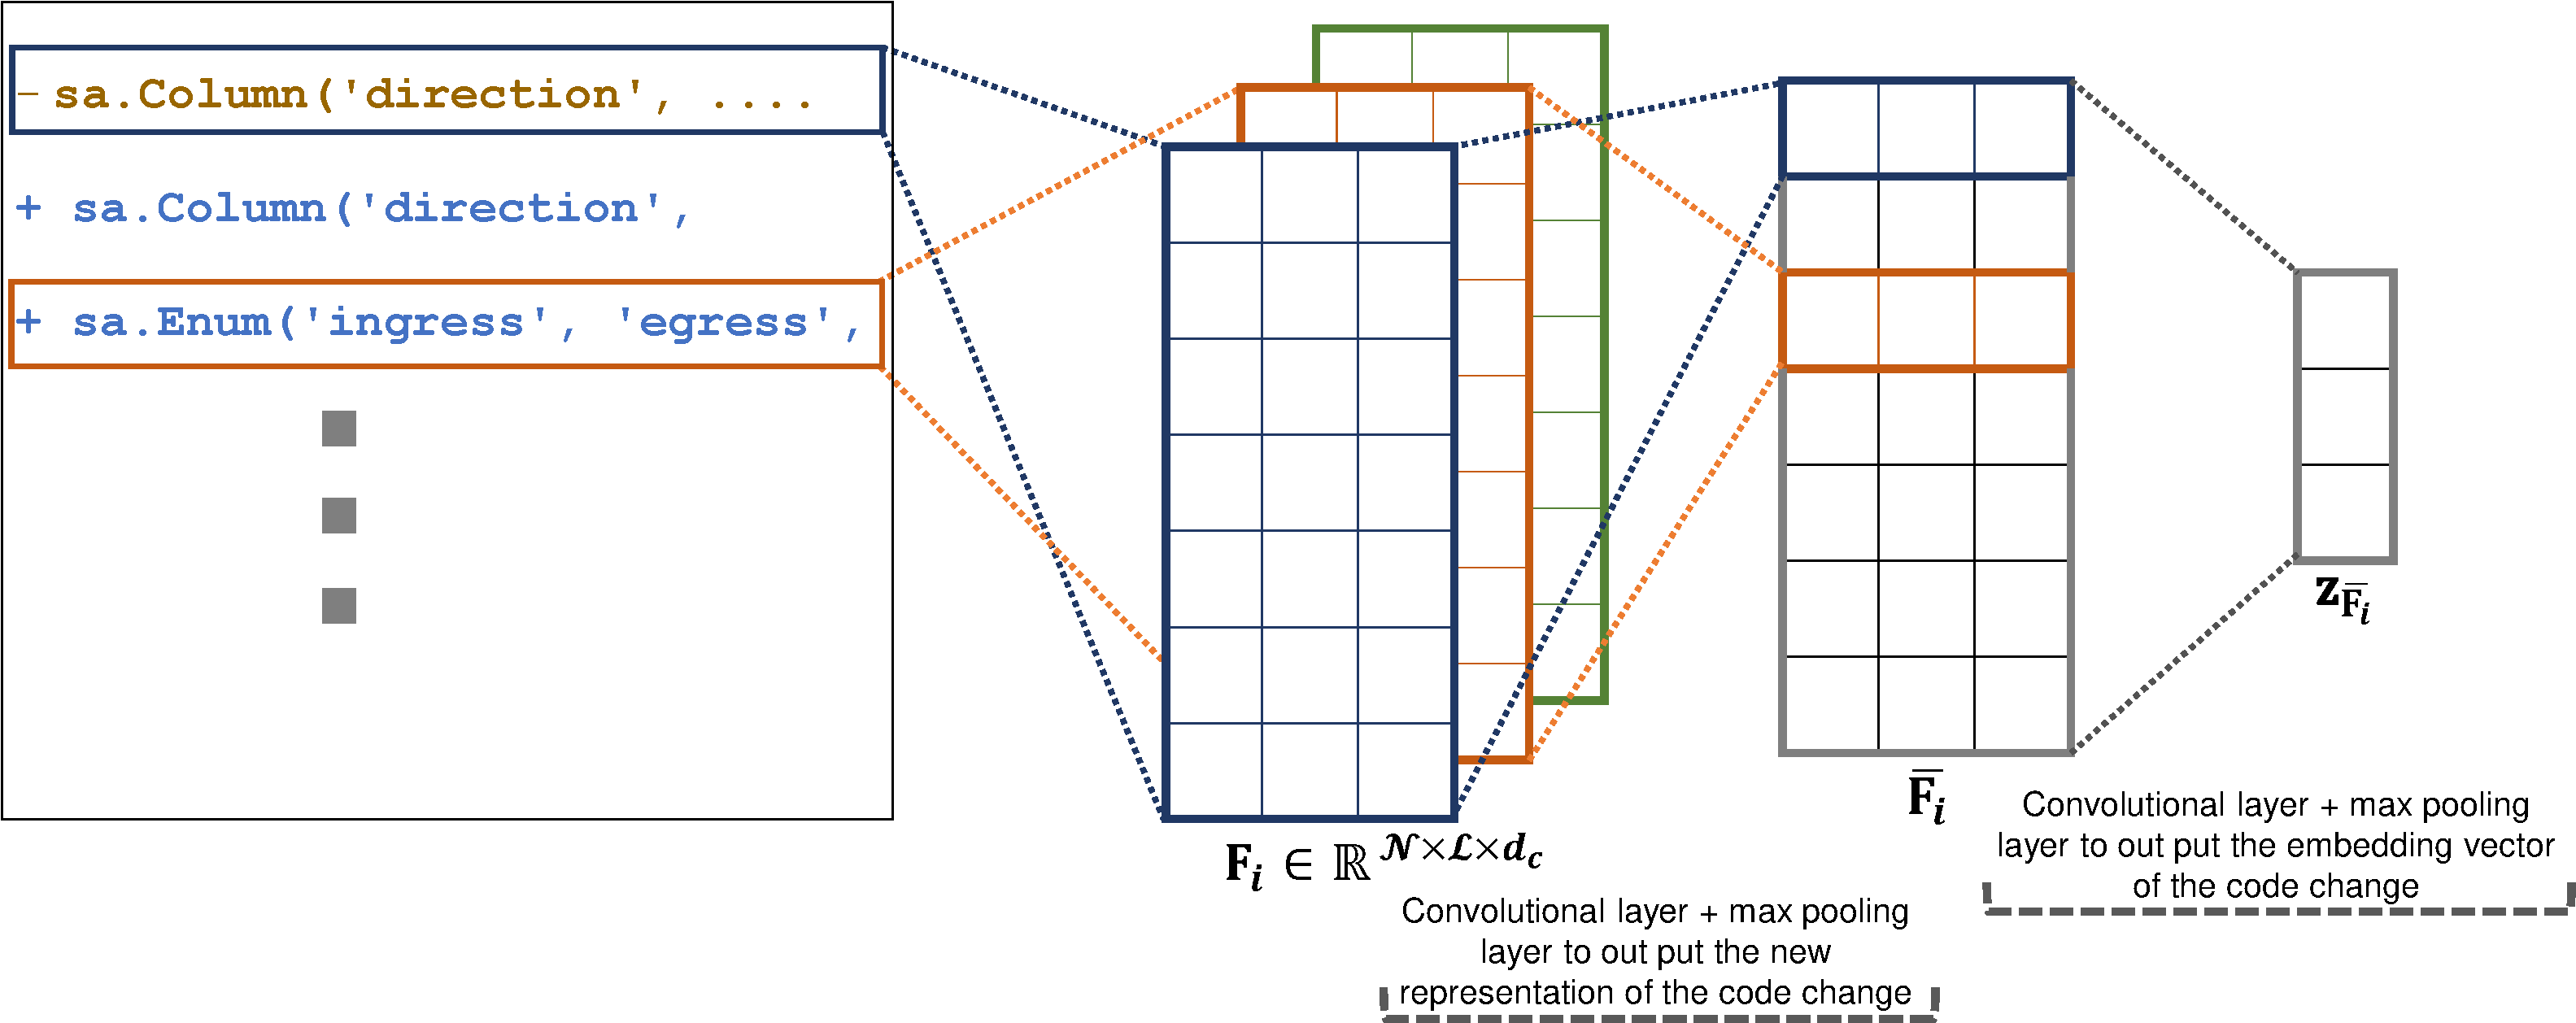
\includegraphics[scale=0.25]{figs/code_framework.pdf}
	\caption{The overall structure of convolutional neural network for each change file in code change. The first convolutional and pooling layers use to learn the semantic features of each added or removed code line based on the words within the added or removed line, and the subsequent convolutional and pooling layers aim to learn the interactions between added or removed code line with respect to the code change structure. The output of the convolutional neural network is the embedding vector $\textbf{z}_{\overline{\textbf{F}}_{i}}$ representing the salient features of the each change file.}
	\label{fig:code}
\end{figure*}

In this section, we focus on building convolutional networks for code changes to solve the just-in-time defect prediction problem. 
Code change, although it can be viewed as a sequence of words, differs from natural language mainly because of its structure. The natural language carries sequences of words, and the semantics of the natural language can be inferred from a bag of words~\cite{ng1997corpus}. On the other hand, the code change includes a change in different files and different kinds of changes (removals or additions) for each file. Hence, to extract salient features from the code changes, the convolutional networks should obey the code changes structure. 
Based on the aforementioned considerations, we propose novel neural networks for extracting silent features from code changes based on convolutional neural networks. 

Given a code change $\mathcal{C}$ including a change in different source code files $[\text{F}_1, \dots, \text{F}_n]$, where $n$ is a number of files in the code change, we aim to extract salient features for each different file $\text{F}_i$. The salient features of each file are then concatenated to each other to represent the features for the given code change. In the rest of this section, we explain how the convolutional networks can extract the salient features for each file in the code change and how these salient features are concatenated. 

Suppose $\text{F}_i$ represents a change in each different file, $\text{F}_i$ contains a number of lines (removals or additions) in a code change file. We also have a sequence of words in each line in $\text{F}_i$. Similar to the section~\ref{sec:cnn_msg}, we first aim to obtain its matrix representation $\text{F}_i \rightarrow \textbf{\text{F}}_i \in \mathbb{R}^{\mathcal{N} \times \mathcal{L} \times{d_c}}$, where $\mathcal{N}$ is the number of lines in a code change file, $\mathcal{L}$ presents a sequence of words in each line, and $d_c$ is a $d_c$-dimensional vector of a word appearing in the $\text{F}_i$. For the purposed of parallelization, all the source code files are padded or truncated to the same $\mathcal{N}$ and $\mathcal{L}$. 

For each line $\mathcal{N}_i \in \mathbb{R}^{\mathcal{L} \times d_c}$, we follow the convolutional network architecture for commit message described in section~\ref{sec:cnn_msg} to extract its embedding vector, called $\textbf{z}_{\mathcal{N}_i}$. The embedding vector $\textbf{z}_{\mathcal{N}_i}$ aims to learn the salient features or the semantic of a code line based on the words within the code line. These features $\textbf{z}_{\mathcal{N}_i}$ are then stacked to produce the new representation of the code change file $\text{F}_i$ as follows: 
\begin{equation}
\label{eq:concatenate}
\overline{\textbf{F}}_{i} = [\textbf{z}_{\mathcal{N}_1}, \dots, \textbf{z}_{\mathcal{N}_{|\mathcal{N}|}}]
\end{equation}

We again apply the convolutional layer and pooling layer on the new representation of the code change (i.e., $\overline{\textbf{F}}_{i}$) to extract its embedding vector, namely $\textbf{z}_{\overline{\textbf{F}}_{i}}$. The $\textbf{z}_{\overline{\textbf{F}}_{i}}$ aims to learn the salient features or the semantics conveyed by the interactions between added or removed lines. Figure~\ref{fig:code} presents an overall convolutional network architecture for each change file $F_i$ in code changes. The first convolutional and pooling layers aim to learn a new representation of the file, and the subsequent convolutional and pooling layers aim to extract the salient features from the new representation of the change file. 

For each change file $\text{F}_i \in C$, we build its embedding vector $\textbf{z}_{\overline{\textbf{F}}_{i}}$. These embedding vectors are then concatenated to build a new embedding vector representing the salient features of the code change $C$ as follows: 
\begin{equation}
\label{eq:concatenate_code}
\textbf{z}_C = \textbf{z}_{\overline{\textbf{F}}_{1}} \oplus \dots \oplus \textbf{z}_{\overline{\textbf{F}}_{n}}
\end{equation}
where $\oplus$ is the concatenation operator. 

%For each line $\mathcal{L}_i$, we follow the convolutional networks described in section~\ref{sec:cnn_msg} to extract its features, called $\textbf{z}_{\mathcal{L}_i}$.

\subsection{Feature Combination}
\label{sec:ftr_combine}
\begin{figure}
	\center
	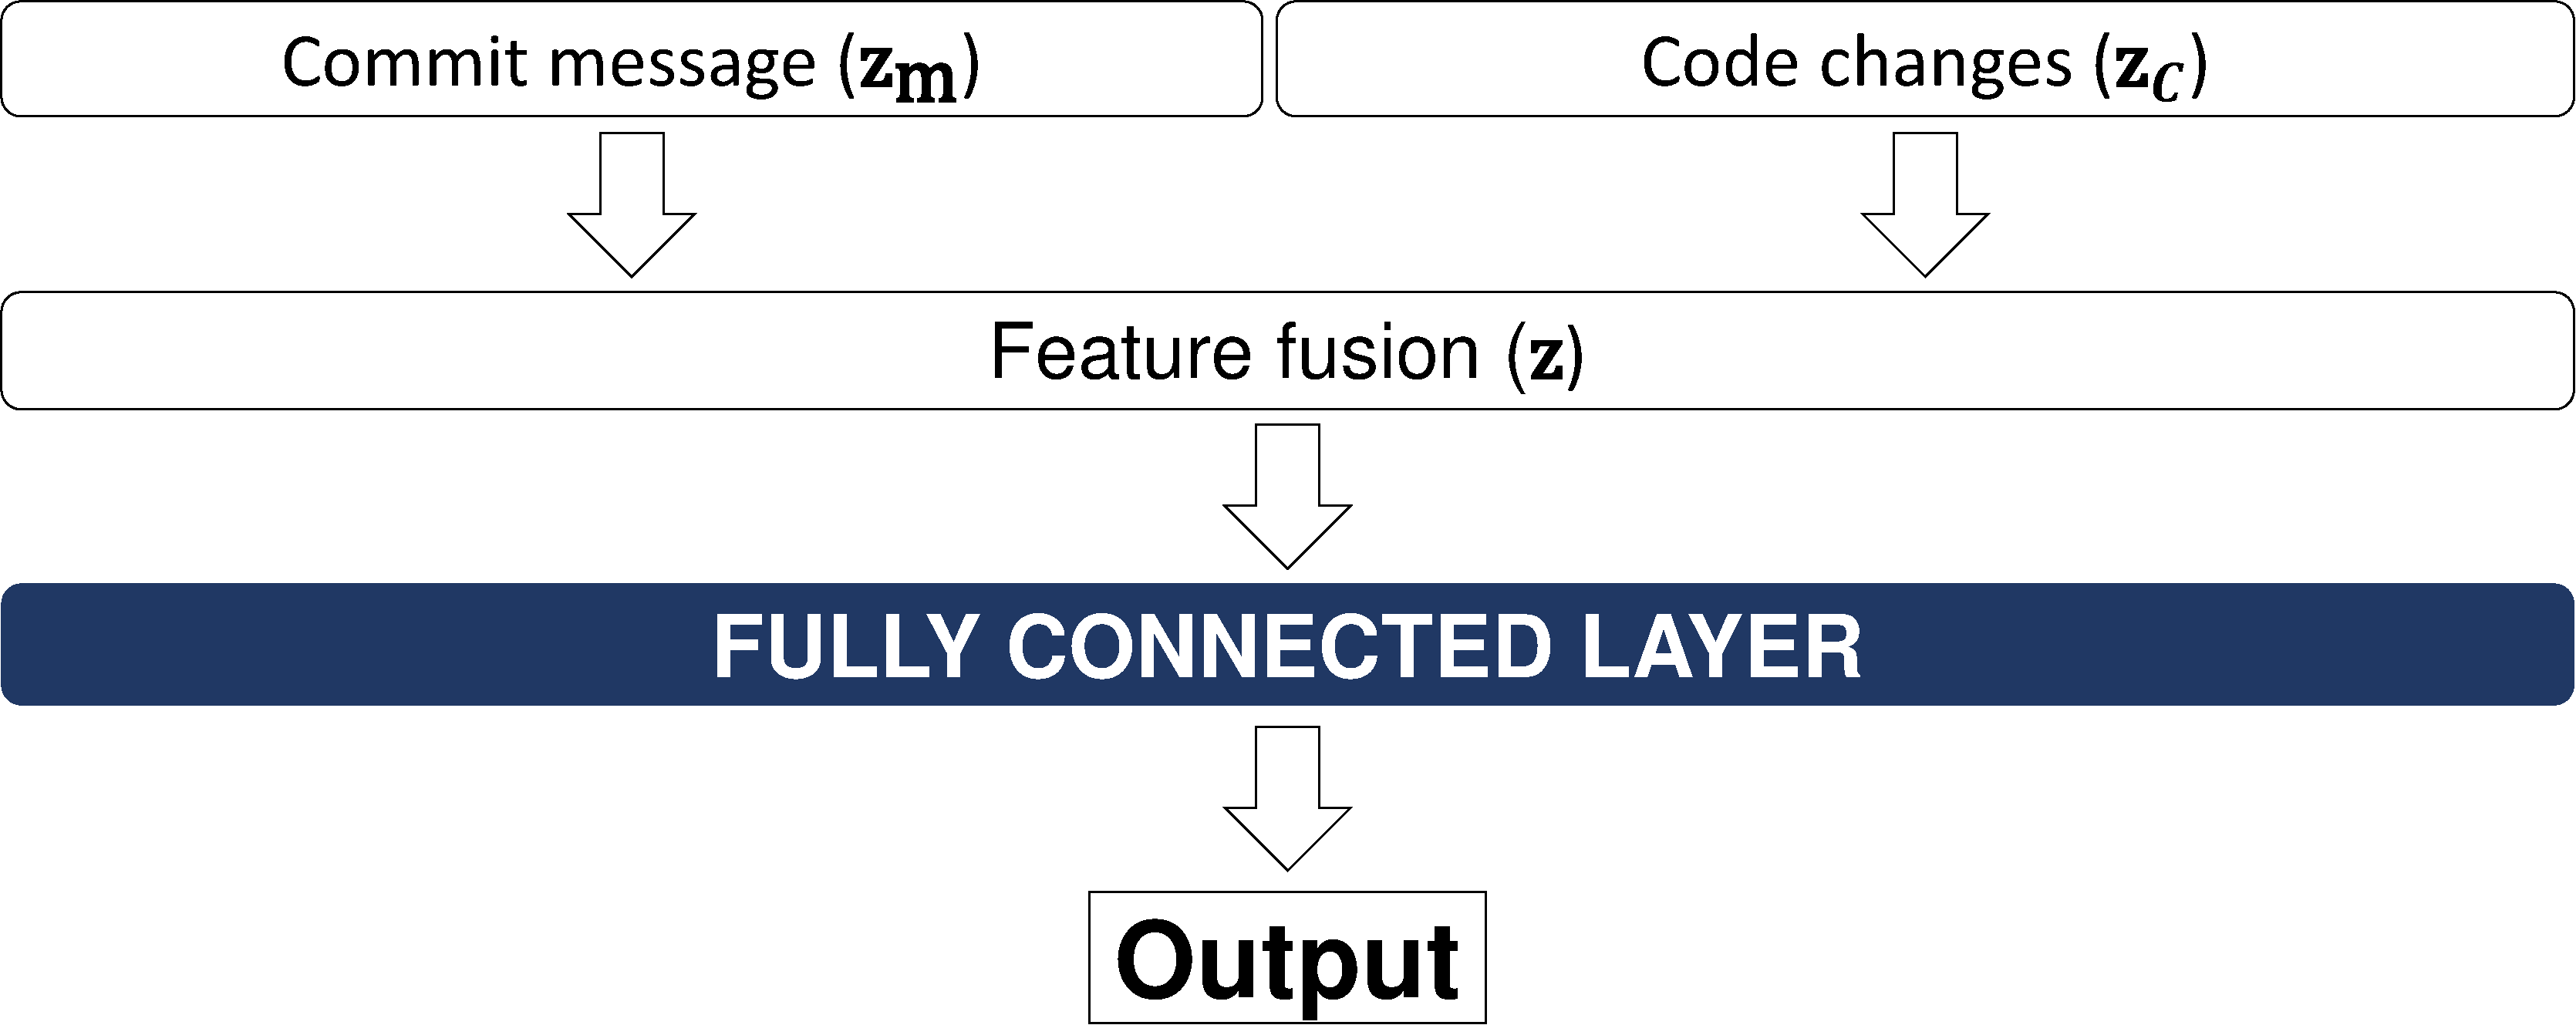
\includegraphics[width=8cm,height=4cm]{figs/code_msg.pdf}
	\caption{The structure of fully-connected network for feature combination. The embedding vector of commit message $\textbf{z}_\textbf{m}$ and code change $\textbf{z}_C$ are concatenated to generate a single vector (i.e., $\textbf{z}$).}
	\label{fig:code_msg}
\end{figure}

Figure~\ref{fig:code_msg} shows the details of architecture of the feature combination. The inputs of this architecture are the two embedding vectors $\textbf{z}_\textbf{m}$ and $\textbf{z}_C$ which represent the salient features extracted from the commit message and code change, respectively. 

These vectors are then concatenated to generate a unified feature representation, i.e., a new vector ($\textbf{z}$), representing the commit change:
\begin{equation}
\label{eq:commit_code}
\textbf{z} = \textbf{z}_\textbf{m} \oplus \textbf{z}_C
\end{equation}

The new vector then feed into a fully-connected (FC) layer, which outputs a vector $\textbf{h}$ as follows:
\begin{equation}  % \footnotesize
\label{eq:fully_layer}
\textbf{h} = \alpha(\textbf{w}_\textbf{h} \cdot \textbf{z} + b_\textbf{h})
\end{equation}
where $\cdot$ is a dot product, $\textbf{w}_h$ is a weight matrix of the vector $\textbf{h}$ and the FC layer, $b_\textbf{h}$ is the bias value, and $\alpha(\cdot)$ is the RELU activation function. The vector $\textbf{h}$ is passed to an output layer to compute a probability score for a given commit:


Finally, the vector $\mathbf{h}$ is passed to an output layer, which
computes a probability score for a given patch:
\begin{equation}  %\footnotesize
p(y_i=1|x_i) = \frac{1}{1 + \exp({-\textbf{h} \cdot \textbf{w}_\textbf{o})}}
\end{equation}
where $\textbf{w}_\textbf{o}$ is the weight matrix between the FC layer and the output layer.

\subsection{Parameters Learning}
\label{sec:learning_parameters}

In the training process, DeepJIT aims to learn the following parameters: the
word embedding matrices of commit messages and commit code in a given commit, the convolutional layers matrices, the weights and bias of
the fully connected layer and the output layer. 

In the \emph{Just-In-Time} defect prediction, only a few commits contain a buggy code while a large number of commits are clean. Such an imbalance nature increases the difficulty in learning a prediction function~\cite{chawla2004special}. Inspired by~\cite{zhou2006training, kukar1998cost}, we propose an unequal misclassification loss function which helps to reduce the negative influence of the imbalanced data. 

Let $\textbf{w}_\textbf{n}$ and $\textbf{w}_\textbf{p}$ are the cost of incorrectly associating a commit change and the cost of missing a buggy commit change, respectively. The parameters of DeepJIT can be learned by minimizing the following objective function:
\begin{equation} %\footnotesize
\label{eq:cost}
\begin{split}
\mathcal{O} &= -\log\left( \prod_{i=1}^{} p(y_i|x_i) \right) + \frac{\lambda}{2} \|\theta\|_{2}^{2} \\
&= -\sum_{i=1}^{} [ \textbf{w}_\textbf{n} (1 - y_i) \log(1 - p(y_i|x_i)) \\ 
&+ \textbf{w}_\textbf{p} y_i \log (p(y_i|x_i)) ] + \frac{\lambda}{2} \|\theta\|_{2}^{2}
\end{split}
\end{equation}
where $p(y_i|x_i)$ is the probability score from the output layer and $\theta$ contains all parameters our model. The term $\frac{\lambda}{2} \|\theta\|_{2}^{2}$ is used to mitigate data overfitting in training deep neural networks~\cite{caruana2001overfitting}. We also apply the dropout technique~\cite{srivastava2014dropout} to improve the robustness of our model. 

We choose Adam~\cite{kingma2014adam}, which is a variant of stochastic gradient descent (SGD)~\cite{bottou2010large}, to minimize the objective function in the equation~\ref{eq:cost}. We choose Adam due to its computational efficiency and low memory requirements compared to other optimization techniques~\cite{kingma2014adam, anthimopoulos2016lung, arora2018optimization}. To efficiently compute the gradients in linear time (with respect to the neural network size), we use backpropagation~\cite{hagan1994training}, which is a simple implementation of the chain rule of partial derivatives.
